\chapter{Introduction}

\noindent This report will evaluate the relative performance of various algorithms for integer factorization, namely Trial Division, Fermat's Factorization, Pollard's Rho Algorithm, Lenstra's Elliptic Curve Factorization Algorithm and briefly the Quadratic Sieve. The algorithms will first be presented to describe how they work. A small example will be included for each algorithm. Then the pseudo code for the algorithm implementations used in the authors' implementations will be presented - along with any methods used solely for that algorithm. Then the method for the gathering of data will be presented. The results will then be presented. Lastly the results and further work will be discussed.

\section{Definitions}

\subsection{Factor and Trivial Factor}
In this paper, a \textit{factor} to a number $n\in\mathbb{N}$ is a number $d\in\mathbb{N}, d\notin\{1, n\}$ so that $d$ evenly divides $n$. A \textit{trivial factor} to a number $n\in\mathbb{N}$ is a number $d\in\{1, n\}$.

\subsection{The Size of Primes}
In this paper, different sizes of primes are mentioned for simplicity's sake. These sizes are \textit{Small}, \textit{Medium}, \textit{Large} and \textit{Larger}. In other cases, the size is made clear by the amount of bits representing the prime.

\textit{Small} primes are primes $p$ such that $2\leq p \leq 100$ (up to $7$ bits). \textit{Medium} primes are primes $p$ such that $1000 \leq p \leq 10000$ (up to $14$ bits). \textit{Large} primes are primes $p$ such that $50000\leq p \leq 100000$ (up to $17$ bits). \textit{Larger} primes are primes $p$ such that $250000\leq p \leq 1000000$ (up to $20$ bits). These sizes are usually mentioned when a number consists of multiple prime factors.

These sizes bear no resemblance to the size of primes usually used in cryptography. The size of primes used in the modern crypto RSA, for example, should use at least $1024$ bit primes until the year of 2030\cite{keysize}.

In this paper, the approximate size of a number in bits was calculated using $\ceil{\log_2{n}},\;n\in\mathbb{N}$.

%%%%
%% TRIAL DIVISION
%%%%
\subsection{Trial Division}
Trial Division is one of the simplest factorization algorithms. The algorithm divides a composite number $n$ by possible factors $p$ in the range $2 \leq p < \floor{\sqrt{n}}$. Usually the factors are tested from either the smallest value to the largest, or the opposite. The values are usually increased by one or to the next odd number\cite{trialDivisionAndFermats}.

To visualize the algorithm, here is how one method of Trial Division factorizes $n=15=3\cdot5$. Note that $\leftarrow$ indicates assignment of a value.

Start off with a possible factor $f=2$. The composite number $n=15$ is not divisible by $2$, therefore $f\leftarrow2+1=3$. The number $n$ is however divisible by $3$, therefore $n\leftarrow n/3=15/3=5$. A factor $3$ has been found and $f\leftarrow3+1=4$. Our remainder $n$ is not divisible by $4$, therefore we increment $f$ once more. At last, $f=5$ divides $n=5$, resulting in $n=1$. The last factor, $5$, has now been found, and since $n=1$ we recognize that there are no more factors and stop. We can conclude that $15=3\cdot5$.

%%%%
%% FERMAT'S FACTORIZATION
%%%%
\subsection{Fermat's Factorization}
Fermat's Factorization method finds the difference of two squares $n = a^2 - b^2$. This method can only factorize odd numbers. To visualize the method, set $a \leftarrow \ceil{\sqrt{n}}$ and $b^2 \leftarrow a^2 - n$. If the square root of $b^2$ is not a whole number, continue the search for the factors. This is done by setting $a \leftarrow a + 1$ and $b^2 \leftarrow a^2 - n$. The factors are then determined by $p = (a + b)$ and $q = (a - b)$ \cite{trialDivisionAndFermats}.

For a more useful understanding of the method let $n=39$. Set $a \leftarrow \ceil{\sqrt{39}}$. Calculate $b^2 \leftarrow 7^2-39 = 10$. Since ten is not a square number set $a \leftarrow 7+1$. Next step is to once more calculate $b^2$ with the new value of $a$. $b^2 \leftarrow 8^2-39 = 25$. $b^2=25 \Rightarrow b=\sqrt{25} = 5$. A square number was found. The factors, $p$ and $q$, are given by $p=(8+5)=13$ and $q=(8-5)=3$ 

%%%%
%% POLLARD'S RHO ALGORITHM
%%%%
\subsection{Pollard's Rho Algorithm}
Pollards Rho ($\rho$) Algorithm for factorization is based on Floyd's detection algorithm for cycles. The basic idea is to iterate a function, $g(x)$ until it falls into a cycle. This function is typically chosen to be $g(x)=x^2+1$. \cite{pollardsRhoAlgorithm}\cite{pollardsRhoAlgorithm2}.

To visualize the algorithm, the factorization of $n=15=3\cdot5$ will be described. Note that $\leftarrow$ indicates assignment of a value.

Let $f=1$, $x=2$, $y=2$ and $g(x)=x^2+1$. Calculate $x=g(x)=g(2)=2^2+1=5$ and $y=g(g(x))=g(g(2))=(2^2+1)^2+1=26$. Since $\gcd(x - y, n)=\gcd(5 - 26, 15)=3$ is not a trivial factor, we have found a factor. The last factor is calculated by dividing $n$ by $3$ resulting in $5$. We can conclude that $15=3\cdot5$.

%%%%
%% LENSTRA'S ELLIPTIC CURVE FACTORIZATION ALGORITHM
%%%%
\subsection{Lenstra's Elliptic Curve Factorization Algorithm}
Lenstra's Elliptic Curve Factorization Algorithm's goal is to find a failure. Since the elliptic curve is not in a group because a prime is not used in the generation of the curve, not all numbers will have a modular inverse \cite{LenstrasFactorizationAlgorithm}. To give a more descriptive view, below is how the algorithm factorizes a number $n$.

Let $n\in\mathbb{N}$ be a composite number and $A, x_1, y_1$ be random elements from $\mathbb{Z}_n \setminus \{0,1\}$. Set $B \leftarrow y_1^2 - x_1^3 - Ax_1\; (\text{mod}\;n)$ and $P_1 = (x_1,y_1)$. If a solution to $P_k$ where $k = \{1,2,...,k_{max}\}$ is not found a  factor to $n$ is found. To decide the next $P$, $\lambda$ is needed. Its given by:

\begin{equation*}
    \lambda = \left\{\begin{array}{l l}
         (3x_1^2 + A)(2y_1)^{-1} & \text{if}\; k = 1\\
         (y_{k-1} - y_1)(x_{k-1} - x_1)^{-1} & \text{if}\; k > 1
    \end{array}\right.
\end{equation*}

Note that the power to the negative one is the modular inverse. If the modular inverse does not exist, a factor has been found. The factor is determined by the $\gcd(x_{k-1}-x_k, n)$. Moreover if the inverse does exist, continue calculating the next $P$. $P_k$ is given by:

\begin{equation*}
    \begin{array}{l}
        x_k =  \left\{\begin{array}{l l}
        \lambda^2 - x_1 - x_1 & \text{if}\; k = 2\\
        \lambda^2 - x_1 - x_{k-1} & \text{if}\; k > 2
        \end{array}\right.\\
        y_k = \lambda(x_1 - x_k) - y_1
    \end{array}
\end{equation*}

And finally $P_k = P_{k-1} + P_1 = (x_k,y_k)$. Repeat the process until the modular inverse can not be calculated.

A more useful way to understand the algorithm is to see an example. This example is taken from "Introduktion till kryptologi" (\cite{Cryptography101}).
Let $n = 35$ and $P = (2,1)$. The elliptic curve is given by $y^2 = x^3 + 4x + 20$.

\begin{equation*}
    \lambda = (3x_1^2 + A)(2y_1)^{-1} = (3*2^2+4)(2*1)^{-1} \equiv 8\pmod{35}
\end{equation*}

Continue by calculating $2P = P + P$.

\begin{equation*}
    \begin{array}{l}
        x_2 = \lambda^2 - x_1 - x_1 = 8^2 - 2 - 2 \equiv 25\pmod{35} \\
        y_2 = \lambda(x_1 - x_2) - y_1 = 8*(2-25) - 1 \equiv 25\pmod{35}
    \end{array}
\end{equation*}

Therefore $2P = (25, 25)$. Sins $2P$ could be calculate. Continue calculating the next point which is $3P$.

\begin{equation*}
    \begin{array}{l}
        \lambda = (y_2 - y_1)(x_2 - x_1)^{-1} = (25-1)(25-2)^{-1} \equiv 33\pmod{35} \\
        x_3 = \lambda^2 - x_1 - x_2 = 33^2 - 25 - 2 \equiv 12\pmod{35}\\
        y_2 = \lambda(x_1 - x_3) - y_1 = 33*(25-12)-25 \equiv 19\pmod{35}
    \end{array}
\end{equation*}

Therefore $3P = (12, 19)$. $3P$ could also be calculated. Continue once more.

\begin{equation*}
    \begin{array}{l}
        \lambda = (y_2 - y_1)(x_2 - x_1)^{-1} = (19-1)(12-2)^{-1}
    \end{array}
\end{equation*}

Calculating $10^{-1}\pmod{35}$ we notice that $\gcd(10,35)=5\neq1$. When the greatest common divider does not equal one, we have found our factor. $35$ was factorized successfully.

%%%%
%% THE QUADRATIC SIEVE
%%%%
\subsection{The Quadratic Sieve}

The Quadratic Sieve is considered one of the fastest integer factorization methods. Not entirely different from Fermat's Factorization method, the Quadratic Sieve algorithm finds values for $a$ and $b$ making $a^2\equiv b^2\;(\text{mod}\;n)$ where $n\in\mathbb{N}$ is the number to factorize \cite{quadraticSieve}. Given $a$ and $b$, two factors $\gcd(a-b, n)$ and $\gcd(a+b, n)$ can be retrieved. Instead of stepping to find the solution like with Fermat's method, the Quadratic Sieve \textit{sieves} its way through. This results in a much faster algorithm. The algorithm generally relies on two parameters, $B$ and $V$. The choice of the parameters are non-trivial \cite{Cryptography101}. Generally $B$ should be close to $L(n)$ where $L(n)$ is the nearest integer to $e^{\sqrt{\ln{n}\cdot\ln{\ln{n}}}}$. The decision of the parameters will heavily impact the capability and performance of the algorithm. The parameter $V$ should generally be between $B$ and $B^2$. Given the complexity of the algorithm and the time required to properly describe the algorithm and provide examples, the authors have decided to refer to E. Landquist (\cite{quadraticSieve}) and R. Nyqvist (\cite{Cryptography101}) for further information.

\subsection{Diagram Format}
The format of the diagrams used in this paper was constructed to be easy to read. Instead of plotting the data, which in its raw format can span several hundred lines, the maximum, average and minimum value is presented.
\begin{figure}[H]
    \centering
    \begin{center}
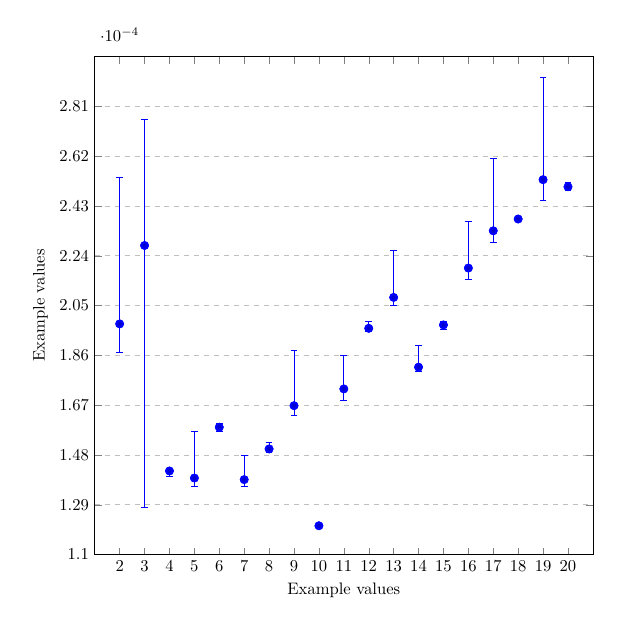
\begin{tikzpicture}[scale=0.6]
\begin{axis}[
    width=1\textwidth,
    height=1\textwidth,
    xlabel={Example values},
    ylabel={Example values},
    xmin=1, xmax=21,
    ymin=0.00011, ymax=0.0003,
    xticklabels={2, 3, 4, 5, 6, 7, 8, 9, 10, 11, 12, 13, 14, 15, 16, 17, 18, 19, 20},
    xtick={2, 3, 4, 5, 6, 7, 8, 9, 10, 11, 12, 13, 14, 15, 16, 17, 18, 19, 20},
    ytick={0.000110000000000000, 0.000129000000000000, 0.000148000000000000, 0.000167000000000000, 0.000186000000000000, 0.000205000000000000, 0.000224000000000000, 0.000243000000000000, 0.000262000000000000, 0.000281000000000000},
    ymajorgrids=true,
    grid style=dashed,
]

\addplot+[
    blue,
    very thick,
    forget plot,
    only marks
    ]
    plot[
    very thick,
    error bars/.cd,
    y dir=plus,
    y explicit
    ]
    table[x=x,y=y,y error expr=\thisrow{y-max}] {
    x    y    y-max
    11	0.0001732	1.28e-05
10	0.000121	1e-06
13	0.0002081	1.79e-05
12	0.0001963	2.7e-06
15	0.0001976	1.4e-06
14	0.0001815	8.5e-06
17	0.0002335	2.75e-05
16	0.0002193	1.77e-05
19	0.000253	3.9e-05
18	0.000238	1e-06
20	0.0002503	1.7e-06
3	0.0002279	4.81e-05
2	0.000198	5.6e-05
5	0.0001392	1.78e-05
4	0.0001419	1.1e-06
7	0.0001386	9.4e-06
6	0.0001586	1.4e-06
9	0.0001668	2.12e-05
8	0.0001503	2.7e-06

    };

\addplot+[
    blue,
    very thick,
    forget plot,
    only marks
    ]
    plot[
    very thick,
    error bars/.cd,
    y dir=plus,
    y explicit
    ]
    table[x=x,y=y,y error expr=\thisrow{y-min}] {
    x    y    y-min
    11	0.0001732	-4.2e-06
10	0.000121	-1e-06
13	0.0002081	-3.1e-06
12	0.0001963	-1.3e-06
15	0.0001976	-1.6e-06
14	0.0001815	-1.5e-06
17	0.0002335	-4.5e-06
16	0.0002193	-4.3e-06
19	0.000253	-8e-06
18	0.000238	-1e-06
20	0.0002503	-1.3e-06
3	0.0002279	-9.99e-05
2	0.000198	-1.1e-05
5	0.0001392	-3.2e-06
4	0.0001419	-1.9e-06
7	0.0001386	-2.6e-06
6	0.0001586	-1.6e-06
9	0.0001668	-3.8e-06
8	0.0001503	-1.3e-06

    };

\end{axis}
\end{tikzpicture}
\end{center}
\end{figure}
The maximum and minimum value is presented with the ends of a vertical line. The average point is presented by a dot.

\section{Purpose}

The purpose of the paper is to validate the performance of various algorithms for integer factorization relative to each other, namely Trial Division, Fermat's Factorization, Pollard's Rho Algorithm, Lenstra's Elliptic Curve Factorization Algorithm and briefly the Quadratic Sieve.

\section{Delimitations}

No effort will be made to optimize the implemented algorithms further than what is considered logical. No algorithm will leverage parallel computing techniques, dynamic programming techniques or other performance gaining techniques. No consideration of performance will be made when choosing software and programming stack.